\documentclass[./../main_file.tex]{subfiles}

\begin{document}
	
	Trong phần này, nhóm sẽ giới thiệu cách cài đặt và sử dụng 3 công cụ của Selenium.
		
	\subsection{Selenium IDE}
	
	Vì Selenium IDE là add-on trên Mozilla Firefox hoặc extension trên Google Chrome, Microsoft Edge nên việc cài đặt Selenium IDE vô cùng đơn giản. Yêu cầu bắt buộc để cài đặt Selenium IDE là máy tính có cài đặt một trong các trình duyệt trên. Nhóm sẽ hướng dẫn các bước cài đặt Selenium IDE trên trình duyệt Google Chrome.
	
	\begin{enumerate}
		\item Tìm kiếm Selenium IDE trên cửa hàng extension của Google Chrome hoặc Firefox (hình \ref{fig:ide_chrome})
		\begin{figure}
			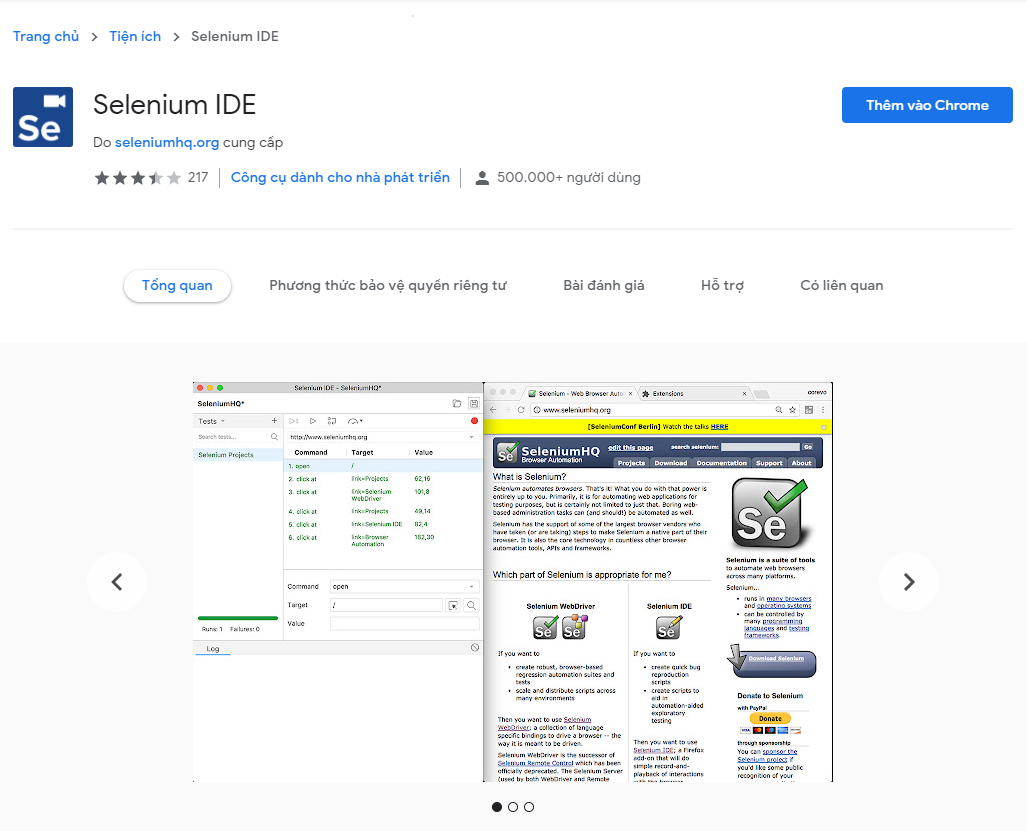
\includegraphics[width=\linewidth]{./images/ide_install.png}
			\caption{Trang của Selenium IDE trên Chrome Web Store}
			\label{fig:ide_chrome}
		\end{figure}
		\item Nhấn “Thêm vào Chrome” để tiến hành cài đặt % (hình \ref{fig:ide_add_to_chrome})
		\item Sau khi cài đặt xong, Selenium IDE sẽ hiển thị trên thanh công cụ. Nhấn vào biểu tượng Selenium IDE để chạy ứng dụng
	\end{enumerate}

	\subsection{Selenium WebDriver}
	
	Trước khi sử dụng được công cụ WebDriver, trình điều khiển cho các trình duyệt như Chrome, Firefox phải được cài đặt. Các trình điều khiển này có thể được tải về trên trang chủ của Selenium. Sau khi tải về, người dùng cần đưa các trình điều khiển vào PATH trên máy tính.
	
	Khi hoàn thành cài đặt trình điều khiển, người dùng có thể bắt đầu cài đặt WebDriver. Công cụ này hỗ trợ nhiều ngôn ngữ lập trình phổ biến, nhưng tài liệu này sẽ chỉ hướng dẫn cài đặt WebDriver cho ngôn ngữ Java. Người dùng có thể cài đặt công cụ này thông qua Maven bằng việc thêm dependency vào file pom.xml trong project Java.
	
	\begin{lstlisting}[language=XML,caption=pom.xml]
		<!--Add this to pom.xml-->
		<dependency>
			<groupId>org.seleniumhq.selenium</groupId>
			<artifactId>selenium-java</artifactId>
			<version>3.X</version>
		</dependency>
	\end{lstlisting}

	\subsection{Selenium Grid}
	
	Để cài đặt Selenium Grid, người dùng cần tải xuống file jar cho chương trình Selenium Server trên trang Downloads của Selenium. Sau đó, người dùng có thể chạy file jar này để cài đặt máy tính của mình với tư cách là một hub hoặc một node.
	
	\begin{lstlisting}[caption=Lệnh để chạy Selenium Server]
		java -jar selenium-server-standalone.jar -role hub
	\end{lstlisting}
	
\end{document}